\section{Distribuciones de tipo gamma}

La familia gamma es una generalización de varias distribuciones importantes
(exponencial, chi-cuadrada, Erlang) y aparece frecuentemente al modelar
\emph{tiempos de espera}.

\subsection{Función gamma}

\begin{definicion}[Función gamma]
La \emph{función gamma} $\Gamma: (0,\infty) \to \mathbb{R}$ se define como
\begin{align}
 \label{eq:2.8.6}
 \Gamma(\alpha) = \int_0^\infty t^{\alpha-1} e^{-t}\,dt.
\end{align}
\end{definicion}

{Propiedades de la función gamma}
\begin{itemize}
 \item $\Gamma(1) = 1$.
 \item $\Gamma(\alpha + 1) = \alpha\,\Gamma(\alpha)$ para todo $\alpha > 0$.
 \item En particular, para $\alpha \in \mathbb{N}$ se cumple
 $\Gamma(n) = (n-1)!$.
 \item $\Gamma(1/2) = \sqrt{\pi}$.
\end{itemize}

\subsection{Distribución gamma}

\begin{definicion}[Distribución gamma]
Una variable aleatoria continua $X$ tiene \emph{distribución gamma} con parámetros
de forma $\alpha > 0$ y escala $\beta > 0$ si su función de densidad es
\begin{align}
 \label{eq:2.8.7}
 f(x) =
 \begin{cases}
  \dfrac{1}{\Gamma(\alpha)\,\beta^\alpha}\,x^{\alpha-1}\,e^{-x/\beta},
  & x > 0, \\
  0, & \text{en otro caso.}
 \end{cases}
\end{align}
Escribimos $X \sim \text{Gamma}(\alpha, \beta)$.
\end{definicion}

{Propiedades de la distribución gamma} Si $X \sim \text{Gamma}(\alpha, \beta)$, entonces
\begin{align}
 \mu_X &= \alpha\beta, \\
 \s_X^2 &= \alpha\beta^2.
\end{align}

\subsection{Distribución exponencial}

La distribución exponencial modela el tiempo de espera hasta la ocurrencia de un evento
cuando los eventos ocurren de manera continua e independiente a una tasa constante (por
ejemplo, el tiempo entre llamadas a un centro de atención, o el tiempo de vida de un
componente electrónico antes de una primera falla).

\begin{definicion}[Distribución exponencial]
Una variable aleatoria continua $X$ tiene \emph{distribución exponencial} con parámetro
de tasa $\lambda > 0$ si su función de densidad es
\begin{align}
 \label{eq:2.8.8}
 f(x) =
 \begin{cases}
  \lambda\,e^{-\lambda x}, & x \geq 0, \\
  0, & \text{en otro caso.}
 \end{cases}
\end{align}
Escribimos $X \sim \text{Exp}(\lambda)$.
\end{definicion}

{Propiedades de la distribución exponencial} Si $X \sim \text{Exp}(\lambda)$, entonces
\begin{align}
 \mu_X &= \frac{1}{\lambda}, \\
 \s_X^2 &= \frac{1}{\lambda^2}.
\end{align}

\begin{observacion}[Propiedad de pérdida de memoria]
La distribución exponencial satisface la \emph{propiedad de pérdida de memoria}:
para $s, t \geq 0$,
\begin{align}
 P(X > s + t \mid X > s) = P(X > t).
\end{align}
Es la única distribución continua (además de la geométrica en el caso discreto)
con esta propiedad.
\end{observacion}

La distribución exponencial con parámetro $\lambda$ corresponde exactamente al caso
particular $\text{Gamma}(1, \beta)$ de la familia gamma, con $\lambda = 1/\beta$. Esta
identificación explica, entre otras cosas, por qué la suma de $n$ variables exponenciales
independientes con la misma tasa sigue una distribución Gamma, como se muestra a
continuación.

\subsection{Caso particular: distribución chi-cuadrada}

La distribución chi-cuadrada con $\nu$ grados de libertad, denotada $\chi^2_\nu$, es
un caso particular de la distribución gamma con parámetros
$\alpha = \nu/2$ y $\beta = 2$:
\begin{align}
 \label{eq:2.8.9}
 X \sim \chi^2_\nu \iff X \sim \text{Gamma}\!\left(\frac{\nu}{2}, 2\right).
\end{align}
Su función de densidad es
\begin{align}
 f(x) = \frac{1}{2^{\nu/2}\,\Gamma(\nu/2)}\,x^{\nu/2-1}\,e^{-x/2}, \qquad x > 0.
\end{align}

Esta distribución ya se estudia en detalle en la sección \ref{sec:3.9} del capítulo
de inferencia; la conexión con la familia gamma permite generalizar varios de sus
resultados.

\subsection{Suma de variables gamma independientes}

\begin{teorema}[Propiedad de suma de gamma]
Si $X_1, X_2, \dots, X_n$ son variables aleatorias independientes con
$X_i \sim \text{Gamma}(\alpha_i, \beta)$ (con la misma escala $\beta$), entonces
\begin{align}
 \label{eq:2.8.10}
 Y = X_1 + X_2 + \cdots + X_n \sim \text{Gamma}\!\left(\sum_{i=1}^n \alpha_i,\, \beta\right).
\end{align}
\end{teorema}

\begin{ejemplo}
 \label{exmp:2.8.3}
Las llamadas a un \emph{call center} llegan siguiendo un proceso de Poisson con tasa
$\lambda = 3$ llamadas por minuto. ¿Cuál es la distribución del tiempo hasta la
tercera llamada? ¿Cuál es la probabilidad de que este tiempo sea mayor a $1.5$ minutos?
\end{ejemplo}

\begin{solucion}
El tiempo entre llamadas consecutivas es exponencial con parámetro $\lambda = 3$, es
decir, $T_i \sim \text{Exp}(3)$ con media $1/3$ minutos.

Por la propiedad aditiva de la distribución gamma, el tiempo hasta la tercera llamada
es
\begin{align}
 T = T_1 + T_2 + T_3 \sim \text{Gamma}(3, 1/3).
\end{align}
Equivalentemente, $T \sim \text{Erlang}(3, 3)$ con parámetro de tasa $3$.

La probabilidad de que $T > 1.5$ es
\begin{align}
 P(T > 1.5) = 1 - F_{\text{Gamma}}(1.5; 3, 1/3) = e^{-3 \cdot 1.5}\left(1 + 3\cdot 1.5 + \frac{(3\cdot 1.5)^2}{2}\right).
\end{align}

Numéricamente: $3 \cdot 1.5 = 4.5$, por lo que
\begin{align}
 P(T > 1.5) = e^{-4.5}\left(1 + 4.5 + \frac{20.25}{2}\right) = e^{-4.5}(15.625) \approx 0.174.
\end{align}
\end{solucion}

\lstinputlisting[language=Python]{../code/distribuciones-continuas-avanzadas/distGamma.py}

\begin{figure}
 \centering
 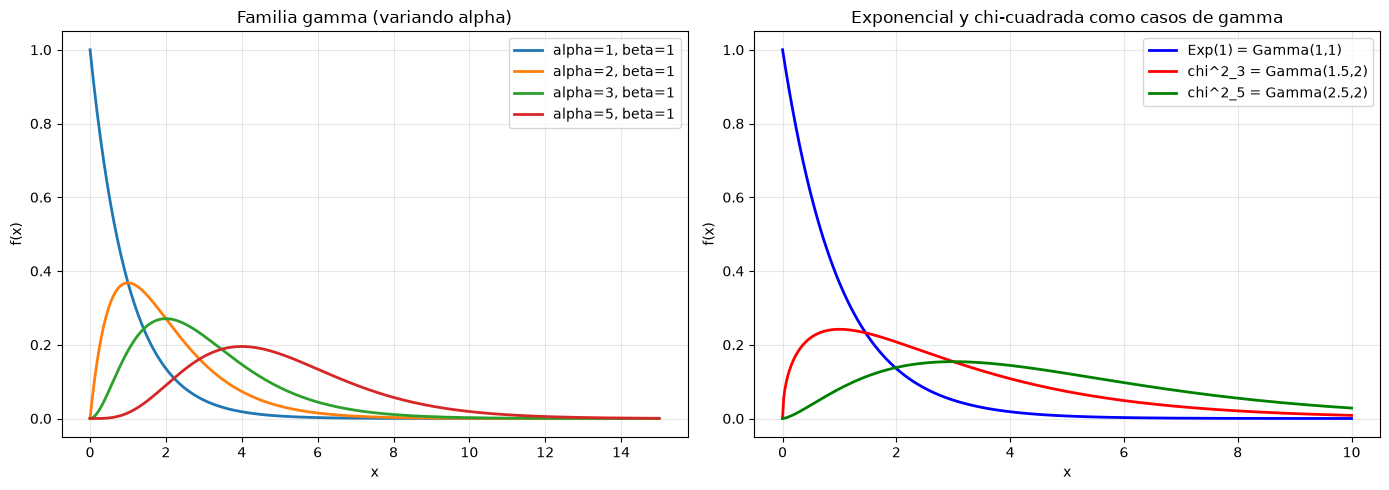
\includegraphics[height=7cm,keepaspectratio=true]{./pe/distGamma.png}
 % distGamma.png: 0x0 pixel, 300dpi, 0.00x0.00 cm, bb=
 \caption{Familia gamma y sus casos particulares (exponencial y chi-cuadrada).}
 \label{fig:2.8.3}
\end{figure}



\subsection{Distribución beta}

La distribución beta modela variables aleatorias continuas restringidas al intervalo
$[0,1]$, lo que la hace ideal para representar proporciones, probabilidades desconocidas
o fracciones. Junto con la función gamma, la función beta es una herramienta clásica
del cálculo que conecta ambas familias de distribuciones.

\begin{definicion}[Función beta]
La \emph{función beta} $B: (0,\infty)\times(0,\infty) \to \mathbb{R}$ se define como
\begin{align}
 \label{eq:2.8.16}
 B(\alpha,\beta) = \int_0^1 t^{\alpha-1}(1-t)^{\beta-1}\,dt
 = \frac{\Gamma(\alpha)\,\Gamma(\beta)}{\Gamma(\alpha+\beta)}.
\end{align}
\end{definicion}

\begin{definicion}[Distribución beta]
Una variable aleatoria continua $X$ tiene \emph{distribución beta} con parámetros de
forma $\alpha > 0$ y $\beta > 0$ si su función de densidad es
\begin{align}
 \label{eq:2.8.17}
 f(x) =
 \begin{cases}
  \dfrac{1}{B(\alpha,\beta)}\,x^{\alpha-1}(1-x)^{\beta-1}, & 0 < x < 1, \\
  0, & \text{en otro caso.}
 \end{cases}
\end{align}
Escribimos $X \sim \text{Beta}(\alpha,\beta)$.
\end{definicion}

{Propiedades de la distribución beta} Si $X \sim \text{Beta}(\alpha,\beta)$, entonces
\begin{align}
 \mu_X &= \frac{\alpha}{\alpha+\beta}, \\
 \s_X^2 &= \frac{\alpha\beta}{(\alpha+\beta)^2(\alpha+\beta+1)}.
\end{align}

\begin{observacion}
Cuando $\alpha=\beta=1$, la distribución beta se reduce a la distribución $U(0,1)$.
Además, por estar acotada en $[0,1]$, la distribución beta es el \emph{prior
conjugado} clásico para el parámetro $p$ de una distribución Bernoulli o Binomial
en inferencia bayesiana: si la creencia inicial sobre $p$ es $\text{Beta}(\alpha,\beta)$
y se observan $k$ éxitos en $n$ ensayos, la creencia actualizada (posterior) es
$\text{Beta}(\alpha+k,\, \beta+n-k)$.
\end{observacion}

\begin{ejemplo}
 \label{exmp:2.8.7}
Un control de calidad reporta que la proporción $X$ de artículos defectuosos en un
lote sigue una distribución $\text{Beta}(2,8)$. ¿Cuál es la proporción esperada de
artículos defectuosos? ¿Cuál es la varianza?
\end{ejemplo}

\begin{solucion}
Como $X \sim \text{Beta}(2,8)$,
\begin{align}
 E(X) = \frac{\alpha}{\alpha+\beta} = \frac{2}{10} = 0.2,
\end{align}
es decir, se espera que el $20\%$ de los artículos sean defectuosos.

La varianza es
\begin{align}
 \text{Var}(X) = \frac{\alpha\beta}{(\alpha+\beta)^2(\alpha+\beta+1)}
 = \frac{2\cdot 8}{10^2 \cdot 11} = \frac{16}{1100} \approx 0.0145.
\end{align}
\end{solucion}



\subsection{Distribución Weibull}

La distribución Weibull generaliza a la distribución exponencial al permitir que la
\emph{tasa de falla} (o \emph{función de riesgo}) varíe con el tiempo, por lo que es
ampliamente utilizada en análisis de confiabilidad y estudios de tiempo de vida de
componentes.

\begin{definicion}[Distribución Weibull]
Una variable aleatoria continua $T \geq 0$ tiene \emph{distribución Weibull} con
parámetro de forma $\beta > 0$ y parámetro de escala $\eta > 0$ si su función de
densidad es
\begin{align}
 \label{eq:2.8.18}
 f(t) =
 \begin{cases}
  \dfrac{\beta}{\eta}\left(\dfrac{t}{\eta}\right)^{\beta-1}
  \exp\!\left[-\left(\dfrac{t}{\eta}\right)^{\beta}\right], & t \geq 0, \\
  0, & \text{en otro caso.}
 \end{cases}
\end{align}
Escribimos $T \sim \text{Weibull}(\beta,\eta)$.
\end{definicion}

Su función de distribución acumulada tiene forma cerrada:
\begin{align}
 \label{eq:2.8.19}
 F(t) = 1 - \exp\!\left[-\left(\dfrac{t}{\eta}\right)^{\beta}\right], \qquad t \geq 0.
\end{align}

{Función de riesgo (tasa de falla)} Para una variable de tiempo de vida $T$ con
densidad $f$ y confiabilidad $R(t) = 1 - F(t)$, la \emph{función de riesgo} se define
como $h(t) = f(t)/R(t)$. Para $T \sim \text{Weibull}(\beta,\eta)$,
\begin{align}
 \label{eq:2.8.20}
 h(t) = \frac{\beta}{\eta}\left(\frac{t}{\eta}\right)^{\beta-1}.
\end{align}

\begin{observacion}
El parámetro de forma $\beta$ determina el comportamiento de la tasa de falla:
\begin{itemize}
 \item Si $\beta = 1$, $h(t)$ es constante y $T \sim \text{Exp}(1/\eta)$ (falla
 aleatoria, sin envejecimiento).
 \item Si $\beta < 1$, $h(t)$ es decreciente (mortalidad infantil: fallas tempranas por
 defectos de fabricación).
 \item Si $\beta > 1$, $h(t)$ es creciente (desgaste: la probabilidad de falla aumenta
 con la edad del componente).
\end{itemize}
\end{observacion}

{Propiedades de la distribución Weibull} Si $T \sim \text{Weibull}(\beta,\eta)$,
entonces
\begin{align}
 \mu_T &= \eta\,\Gamma\!\left(1 + \frac{1}{\beta}\right), \\
 \s_T^2 &= \eta^2\left[\Gamma\!\left(1 + \frac{2}{\beta}\right)
 - \Gamma\!\left(1 + \frac{1}{\beta}\right)^2\right].
\end{align}

\begin{ejemplo}
 \label{exmp:2.8.8}
El tiempo de vida $T$ (en miles de horas) de un componente electrónico sigue una
distribución $\text{Weibull}(\beta=2, \eta=5)$. ¿Cuál es la probabilidad de que el
componente falle antes de las $3000$ horas? ¿La tasa de falla es creciente o
decreciente?
\end{ejemplo}

\begin{solucion}
Como $T \sim \text{Weibull}(2,5)$ (con $T$ en miles de horas), buscamos $P(T < 3) =
F(3)$:
\begin{align}
 F(3) = 1 - \exp\!\left[-\left(\frac{3}{5}\right)^2\right]
 = 1 - e^{-0.36} \approx 1 - 0.6977 = 0.3023.
\end{align}
Por lo tanto, hay aproximadamente un $30.23\%$ de probabilidad de falla antes de las
$3000$ horas.

Como $\beta = 2 > 1$, la tasa de falla $h(t) = \frac{2}{5}\left(\frac{t}{5}\right)$ es
\emph{creciente}: el componente presenta un patrón de desgaste, con mayor riesgo de
falla conforme envejece.
\end{solucion}


